%% ------------------------------------------------------------------------- %%
\chapter{Resultados Encontrados e Discussão}
\label{cap:discussao}

\section{Particularidades da execução}

Como os estudos foram executados fisicamente em muitas das empresas selecionadas,
nós acabamos por ajudar na organização do ambiente, mesmo a equipe tendo 
recebido o caderno de questões, com as instruções da instalação
alguns dias antes. A ideia era também gravar a implementação dos alunos,
mas dificuldades em se encontrar um software de vídeo para as diferentes
plataformas, e arquivos muito grandes, impossibilitaram a gravação.

Todos os participantes eram avisados de que tinham por volta de 50 minutos
por exercício. Eles também sabiam que, mesmo que não terminassem o exercício,
deveriam focam sempre na qualidade do código gerado. Eles também eram solicitados
a implementar um design flexível para os problemas. A frase que dizíamos para
eles era geralmente: \textit{"Levem os exercícios para o mundo real, onde um outro
desenvolvedor deverá manter o código gerado. Lembrem-se de implementar o código mais fácil possível
para evoluir. As regras de negócio que existem hoje no enunciado tendem a aumentar
de número e, portanto, deixem a manutenção do código de vocês mais simples."}

Durante a execução, nós tirávamos diversas dúvidas sobre enunciados dos
exercícios, e até mesmo sobre procedimentos que os participantes podiam
adotar durante a execução. Um deles, por exemplo, perguntou se poderia
refatorar o código durante a implementação sem TDD. 
Nós também não os pressionávamos em nenhum momento. Eles ficavam,
cada um suas máquinas, trabalhando na implementação. Não ficávamos 
passando atrás das máquinas para ver como estavam indo, na tentativa
de evitar qualquer possível alteração de comportamento pela nossa presença.
Ao final de cada intervalo de 50 minutos, nós avisámos para eles finalizarem
a linha de raciocínio e partir para o próximo exercício.
Apesar de não haver nenhuma restrição explícita sobre isso, não houveram
conversas entre os participantes. Todos eles trabalharam sozinho
durante toda a implementação.

Todo o experimento ocorreu bem, com exceção do que foi executado
dentro da universidade. Além de diversos problemas de infra-estrutura,
como a falta de espaço disponível para alguns alunos, que impedia até mesmo
o JUnit de executar, todos os participantes conseguiram fazer apenas
1 exercício. Diante desta situação, optamos por deixá-los implementar
o mesmo exercício até o final da aula já que, após os 50 minutos iniciais,
nós observamos que pouco código havia sido escrito. Outro problema levantado
foi que alguns alunos não se mostraram muito dispostos a participar
do estudo.

Ao contrário, a grande maioria dos participantes da indústria conseguiram
implementar o exercício no tempo delimitado, e todos se mostraram
muito receptivos para o estudo. Um ponto que se mostrou bem útil
para convencer participantes da indústria a participar foi a proposta
posterior de nós apresentarmos os resultados encontrados em uma palestra.

Ao final da execução do estudo em cada empresa, nós colhetávamos
os dados gerados (código-fonte e caderno de questões assinado),
e dávamos o nome da pasta do participante, de acordo com
o seguinte formato: \textit{id-nome-combinação}. O id aponta
para um número único do participante no estudo, e a combinação
aponta quais exercícios ele resolveu, bem como em qual deles
ele utilizou TDD.

As entrevistas foram, em grande parte, realizadas pessoalmente com 
o desenvolvedor. Quando o participante não estava disponível (por estar
localizado em outra cidade), a entrevista era realizada por Skype.
Durante toda a entrevista, o participante podia observar o código que
produziu. Para isso, nós criamos uma simples aplicação web para facilitar
a exibição dos códigos-fonte. O objetivo do participante ver o código
era lembrar sobre suas decisões, e nos possibilitar perguntas específicas
sobre o design de classes gerado.

Em média, as entrevistas levavam 30 minutos. Quando o participante comentava
algo interessante, nós fugíamos do roteiro para permitir que ele falasse mais do assunto,
e anotávamos o ponto para que, ao final, fosse possível discutir novamente sobre o assunto.
O roteiro de entrevistas sofreu uma pequena mudança ao final da primeira entrevista,
já que percebemos que comunicar ao participante que o código que ele produziu
\textit{não apresenta um bom design de classes} não era uma tarefa fácil, e talvez, não ética. 
Optamos por perguntar sobre como aquele design de classes foi construído, mesmo que ele
não estivesse bem construído.

Para manter um padrão, nós sempre perguntávamos primeiro sobre o exercício que ele
fez com TDD, independente da ordem que ele implementou no dia da execução. Notamos
que muitos participantes discutiram sobre os exercícios e possíveis implementações com seus colegas.

Dos três especialistas convidados a avaliar os códigos produzidos, apenas um não
completou a tarefa. Sugerimos a todos eles, antes do início da avaliação, que avaliassem
não só a quantidade de código escrito, mas as decisões de design tomadas por aquele
participante. Para que os especialistas avaliassem cada código gerado, nós implementamos
uma simples aplicação web, onde eles tinham acesso a qualquer momento, e podiam parar ou continuar
a avaliar a hora que preferissem.

\section{Descrição dos participantes}

Conforme mencionado, o estudo foi executado em dois ambientes diferentes: em empresas de software
do mercado brasileiro e na academia. Como ambos estudos foram executados de maneira independente,
descrevemos os grupos separados nas sub-seções \ref{findings-desc-industria} e \ref{findings-desc-academia}.

\subsection{Participantes da Indústria}
\label{findings-desc-industria}

Ao todo tivemos 25 participantes, de 6 diferentes empresas.
Os participantes da indústria, em sua maioria, são pessoas com pouca experiência em TDD.
40\% deles disseram utilizar a prática há no máximo um ano. 52\% deles praticam TDD
entre 1 e 3 anos. Apenas 4\% pratica entre três e quatro anos, e nenhum participante
possui mais experiência do que isso. Na Figura \ref{fig:exp-tdd-industria}, mostramos
a distribuição da experiência da prática de TDD entre os participantes.

Os números são um pouco diferentes quando se trata da experiência em desenvolvimento
de software. Por volta de 24\% dos participantes desenvolve software entre 4 e 5 anos.
28\% deles faz isso entre 6 e 10 anos. Entretanto, 20\% possui até 2 anos de experiência.
Na Figura \ref{fig:exp-sw-industria}, mostramos a distribuição.

Entrando em aspectos mais técnicos, 64\% dos participantes afirmam conhecer Java. Entretanto,
36\% dizem não trabalharem com Java no seu dia-a-dia. Todos eles afirmam conhecer JUnit,
e só 12\% diz nunca ter ouvido falar sobre o conceito de objetos dublês. De fato, 64\% deles
aplicam objetos dublês durante suas atividades de desenvolvimento. Com relação a conhecimentos
em orientação a objetos, na pergunta aberta do questionário, grande parte deles 
afirmaram que possuem uma boa experiência e alguns
chegam até a afirmam que dominam o assunto. Poucos disseram que possuem conhecimentos
básicos. Na Tabela \ref{tab:exp-industria},
apresentamos o conhecimento dos participantes em relação a Java, JUnit e objetos dublês.

Esses dados nos mostram que a amostra selecionada se assemelha ao mundo real, onde
encontramos desde desenvolvedores mais experientes até novatos. Em relação a experiência com TDD,
podemos afirmar que metade dos participantes ainda está experimentando a prática, enquanto
outros já a tem mais consolidada. Isso é positivo, já que foi possível capturar informações
da prática de TDD por pessoas com diferentes níveis de maturidade.

Em relação ao alto número de pessoas que não utilizam Java, isso se deve ao fato de uma das
empresas fazer uso de PHP para seu trabalho do dia-a-dia. No entanto, nós conhecemos a equipe
e verificamos que, apesar de não utilizarem a linguagem constantemente, eles não tiveram
problema algum durante a execução dos exercícios.

\begin{figure}[h!]
  \centering
  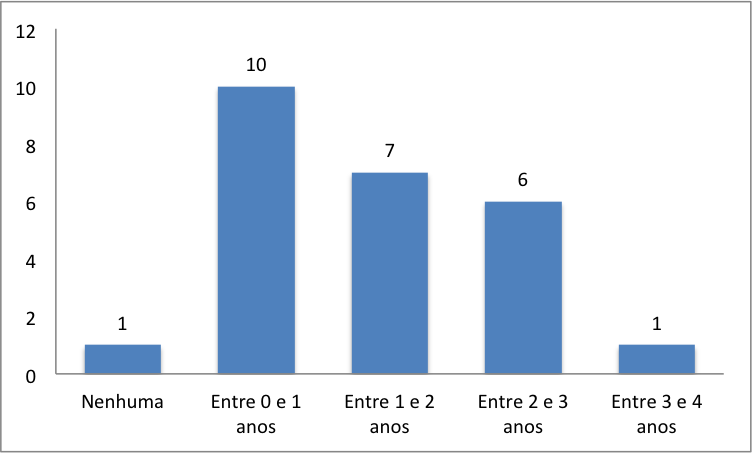
\includegraphics[scale=0.5]{findings/experiencia-tdd-industria.png}
  \caption{Experiência da equipe da indústria com TDD}
  \label{fig:exp-tdd-industria}
\end{figure}

\begin{figure}[h!]
  \centering
  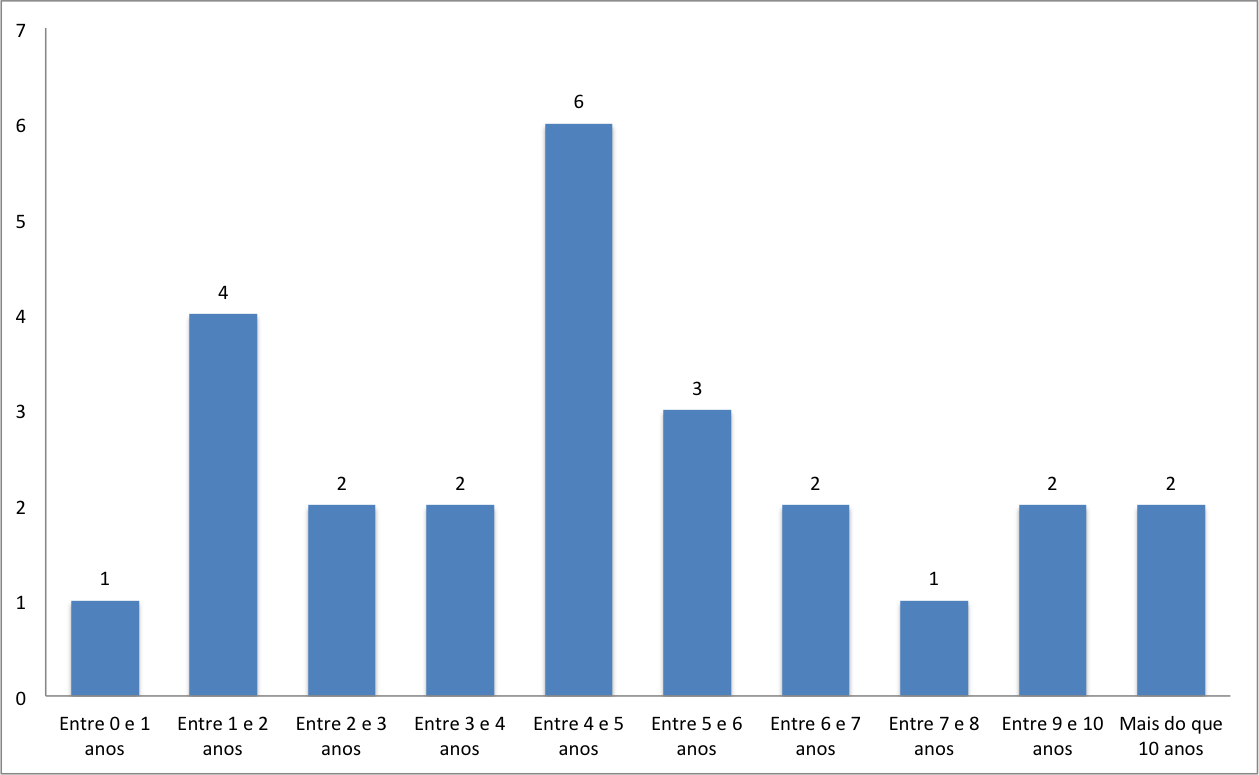
\includegraphics[scale=0.5]{findings/experiencia-sw-industria.png}
  \caption{Experiência da equipe da indústria com desenvolvimento de software em geral}
  \label{fig:exp-sw-industria}
\end{figure}

\subsection{Participantes da Academia}
\label{findings-desc-academia}

Os participantes da academia que participaram do estudo, 21 no total, possuem baixíssima experiência,
tanto em TDD quanto em desenvolvimento de software em geral. Surpreendentemente, 90\%
dos participantes afirmaram não conhecer Java, e 61\% disseram não conhecer TDD.
Em contraste com essa informação, todos eles afirmaram conhecer JUnit, e 76\% afirmaram
conhecer objetos dublês na teoria. 
Na Figura \ref{fig:exp-tdd-academia}, mostramos a experiência dos participantes em TDD, e
na Tabela \ref{tab:exp-academia} apresentamos a experiência deles em Java, JUnit, e objetos
dublês.

Em relação a experiência de desenvolvimento de software, apenas 23\% afirmaram não
ter nenhuma experiência, enquanto que por volta de 43\% afirmaram possuir
entre 2 a 4 anos de experiência. Nenhum participante com experiência superior a isso.
Na Figura \ref{fig:exp-sw-academia}, mostramos a distribuição por completo.

De acordo com os dados, percebemos que grande parte dos participantes não conhecem a linguagem ou
mesmo a prática de TDD. A linguagem foi realmente um problema: durante a execução, percebemos
que muitos deles faziam buscas por elementos simples da linguagem Java, como manipulação de arrays
e listas, ou mesmo por manipulação de texto.

Isso explica o baixo desempenho dos alunos da academia durante
o experimento. Nenhum deles conseguiu terminar os dois exercícios propostos. Por esse
motivo, nenhum aluno foi selecionado para o processo de entrevista. Entretanto,
os códigos-fonte produzidos serão utilizados no processo de análise quantitativa.

\begin{figure}[h!]
  \centering
  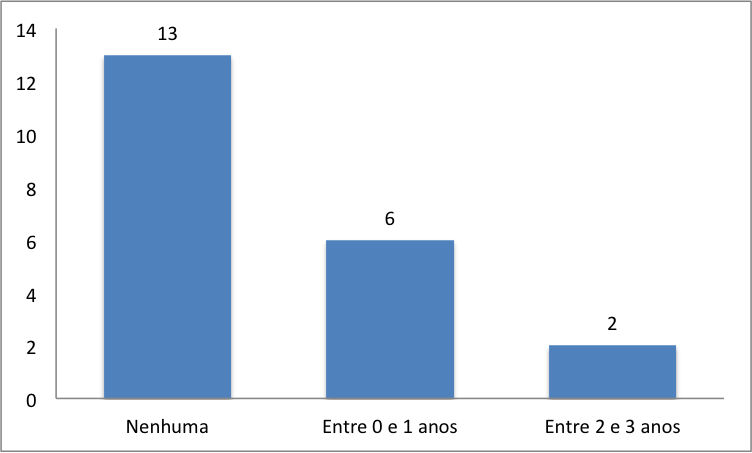
\includegraphics[scale=0.5]{findings/experiencia-tdd-academia.png}
  \caption{Experiência dos estudantes da academia com TDD}
  \label{fig:exp-tdd-academia}
\end{figure}

\begin{figure}[h!]
  \centering
  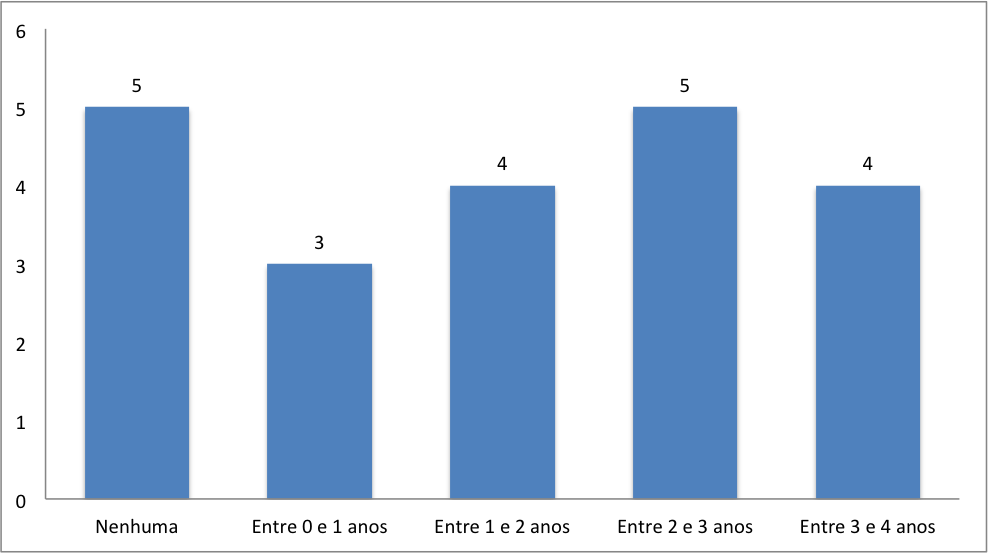
\includegraphics[scale=0.5]{findings/experiencia-sw-academia.png}
  \caption{Experiência dos estudantes da academia com desenvolvimento de software em geral}
  \label{fig:exp-sw-academia}
\end{figure}


\begin{table}
	\begin{tabular}{ | p{5cm} | p{5cm} | p{5cm} | }
		\hline
		Ferramenta & Participantes que conhecem & Participantes que não conhecem\\
		\hline
		Java & 16 & 9\\
		JUnit & 25 & 0\\
		Objetos Dublê & 16 (utilizam no dia-a-dia), 6 (na teoria) & 3\\
		\hline
	\end{tabular}
	\caption{Experiência em Java, JUnit, e Objetos Dublê dos participantes da indústria}
	\label{tab:exp-industria}
\end{table}

\begin{table}
	\begin{tabular}{ | p{5cm} | p{5cm} | p{5cm} | }
		\hline
		Ferramenta & Participantes que conhecem & Participantes que não conhecem\\
		\hline
		Java & 2 & 19\\
		JUnit & 21 & 0\\
		Objetos Dublê & 2 (utilizam no dia-a-dia), 16 (na teoria) & 3\\
		\hline
	\end{tabular}
	\caption{Experiência em Java, JUnit, e Objetos Dublê dos participantes da academia}
	\label{tab:exp-academia}
\end{table}

\section{Inspeção do Código-Fonte}

Nós avaliamos cada código-fonte manualmente.
Em sua maioria, os códigos eram claros e fáceis de entender,
com classes, métodos e variáveis bem nomeados.
Mas, para nossa surpresa,
poucos foram os participantes que fizeram uso de polimorfismo. A grande
maioria das implementações fazia uso de cadeias de condições para 
alcançar o objetivo.

Nós também não conseguimos identificar, de olho, quais códigos
eram produzidos com DGT e quais não eram pois, independente
da prática utilizada, ambos eram muito semelhantes.
De todos os códigos da indústria, apenas um foi completamente eliminado:
um dos participantes não conseguiu nem começar a implementação. Suas classes
eram completamente vazias. 

\section{Análise das Entrevistas}

Diferente do que muitos estudos de TDD afirmam, os participantes, em sua grande maioria, afirmaram que 
a prática de TDD não faria com que o design de classes fosse de alguma forma diferente, caso tivessem
feito ambos os exercícios com a prática.
A principal justificativa dada pelos participantes foi que a experiência e o conhecimento prévio
em orientação a objetos os guiaram durante o processo de criação do design de classes. Nenhum dos
participantes, por exemplo, afirmou que um desenvolvedor sem conhecimento em alguma das áreas
citadas criaria um bom design de classes somente por praticar TDD.

Dois bons exemplos foram dados pelos participantes, que ajudam a reforçar esse ponto. Um deles
comentou que fez uso de um padrão de projetos \cite{gof} que aprendeu apenas alguns dias atrás.
Outro participante mencionou que seus estudos sobre os princípios SOLID (discutidos no Capítulo \ref{cap:design})
o ajudaram durante os exercícios. Segue o trecho mencionado pelo participante:
\textit{"Até foi engraçado, eu estou lendo o Design Patterns (livro), e ele fala de polimorfismo, e foi
lá que eu mirei pra fazer, porque eu nunca tinha feito nada assim (...), aqui dificilmente eu crio
coisa nova, só dou manutenção no código."}

Além do mais, o único participante da indústria que nunca havia
praticado TDD afirmou que não sentiu diferença nenhuma no processo de criação de classes durante
a prática.
Curioso é que esse mesmo participante que nunca praticou TDD afirmou que "sabia que TDD era uma prática de design",
diferentemente dos participantes mais experientes que sempre afirmavam que TDD não é só uma prática de design,
mas também de testes. Isso indica, de certa forma, que a popularidade dos efeitos de TDD no design, por mais
que nada tenha sido provado, é grande.

Quando perguntados sobre o que é TDD, muitos dos participantes lembraram sobre
os efeitos da prática na qualidade externa e a segurança que isso traz
ao desenvolvedor.
Uma frase que exemplifica isso foi dita por um dos participantes:
\textit{"[TDD] acho que tem muita relação com qualidade do código e testes 
de regrassão. Acho que as duas principais vantagens que eu tenho quando uso TDD é isso: o código
fica melhor e depois eu tenho a segurança dos testes de regressão para refatorar."}

Entretanto, apesar do TDD não guiar o desenvolvedor diretamente para um bom design,
todos eles afirmaram que enxergam benefícios na prática de TDD, mesmo do
ponto de vista de design. Muitos deles, inclusive mencionaram a dificuldade
de parar de usar TDD:
\textit{"Você vai fazer alguma coisa, você acaba pensando já nos testes que você vai fazer. É difícil 
falar assim: "programa sem pensar nos testes!" Depois que você acostuma, você não sabe outra
maneira de programar..."} e \textit{"É complicado se disciplinar [a praticar TDD], mas conforme vai passando o tempo, 
você percebe que a curva para se manter o projeto fica bem menos íngreme, 
começa a perceber os benefícios e aí vicia. Você acaba não se sentindo
mais confortável de escrever código sem teste."}

Segundo eles, TDD pode ajudar no processo de design de classes, mas, para isso,
o desenvolvedor deve possuir certa experiência em desenvolvimento de software
para que isso aconteça. Grnade parte dos participantes afirmaram que o 
design de classes criado surgiu de experiências e aprendizados passados.
Segundo eles, a melhor opção é unir a prática de TDD com a experiência:
\textit{"O ideal é somar as duas coisas [experiência e TDD] (...) 
Não acredito que TDD sozinho consiga fazer as coisas ficarem boas. Tem outros conceitos
para as coisas ficarem boas."}

Nas sub-seções abaixo, apresentamos cada um dos pontos 
levantados pelos participantes, bem como discutimos sobre o tópico.

\subsection{Segurança na refatoração}

Os participantes afirmaram que, durante o processo de criação de design, a mudança de ideia é
constante, afinal pouco se conhece do problema, e de como a classe deve ser construída. Segundo eles,
uma vantagem íntriseca do TDD é a suíte de testes gerada. Essa suíte possibilita ao desenvolvedor
muda de ideia e refatorar todo o design de classes com segurança.
A segurança, segundo eles, é fator importante para mudanças de design de classes ou mesmo de implementação:
\textit{"Sim, me dá a chance de aprender pelo caminho e fazer algumas coisas diferentes. (...) O teste te dá segurança."}

Um participante inclusive mencionou uma experiência real, onde o TDD fez a diferença. Segundo ele,
em muitos momentos ele mudava completamente de ideia sobre a implementação, e confiava na bateria
de testes para garantir que o comportamento esperado:
\textit{"No TCC da pós, eu estava desenvolvendo uma ferramenta que trabalhava com manipulação de código, e fiz
tudo com TDD. Várias vezes eu chegava a apagar todo código do sistema, mantinha os testes, e começava uma nova
linha de raciocínio. Achei que me ajudou muito fazer TDD (...), tanto que no fim que eu fui executar a ferramenta,
antes eu só validava pelos testes."}

Novamente, experiência é fator fundamental. Para buscar um código melhor durante a refatoração,
desenvolvedores devem fazer uso de suas experiências:
\textit{"(...) se você não tiver embasamento sobre esses aspectos de única responsabilidade,
coesão, acoplamento, acho que não adianta muito [fazer TDD]. Você precisa ter isso em mente
para conseguir mudar, precisa desse conhecimento para conseguir refatorar."}

\subsection{Passos menores e simplicidade}

TDD sugere que o programador dê sempre pequenos passos (conhecidos pelo termo em
inglês, \textit{baby steps}): deve-se escrever testes sempre para a menor
funcionalidade possível, escrever o código mais simples que faça o teste passar
e fazer sempre apenas uma refatoração por vez \cite{TDDByExample}.

Uma justificativa para tal é a de que, quanto maior o passo que o programador dá, mais
tempo ele leva para concluí-lo e, consequentemente, ele fica mais tempo
sem \textit{feedback} sobre o código. Além disso, faz com que o programador não crie
soluções mais complexas do que elas precisam ser, tornando o código, a longo
prazo, o mais simples possível.

Manter o design de classes simples não é tarefa fácil, e TDD sugere que o programador
escreva sempre o código mais simples que atenda a necessidade. Somente se a
necessidade crescer, é que o programador deverá evoluir o \textit{design}. Uma decisão de
\textit{design} pode ser mais complicada do que parece e, sem um teste para mostrar isso
rapidamente, o programador dificilmente perceberia o problema \cite{aim-fire}.

Todas essas afirmações podem ser validada pela observação de vários participantes sobre o assunto.
Um deles comentou que,
ao não fazer teste, o programador pensa no design de classes de uma só vez, criando, por vezes,
estruturas mais complexas do que o necessário. Isso faz com que ele perceba mais tardiamente
possíveis problemas no desenho inicial:
\textit{"Porque sem os testes, nós não pensamos em passos menores, mas sim na solução inteira
e acaba por não observar problemas que podem acontecer pelo caminho."}

Um dos participantes deixou bem claro como ele faz uso dos \textit{baby steps}, e como
isso o ajuda a pensar melhor no design de suas classes:
\textit{"Porque nós começamos a pensar no pequeno e não no todo. Quando faço TDD eu escrevo
uma regra simples (...), aí vou lá e escrevo o método. Se passou, passou! Como você vai aos poucos,
a arquitetura vai ficando legal. (...) Eu tinha mania de pensar no todo (...), as vezes
em vez de você pensar em um negócio pequeno, você pensa em um enorme. Acho que o cérebro funciona
melhor quando você pensa pequeno. Se você pensa grande, pra mim é óbvio que você vai deixar
alguma coisa faltando."}

Essa afirmação vai de encontro ao discurso comum das metodologias ágeis.
Equipes que seguem as ideias ágeis optam por não fazer o chamado \textit{big design up-front (BDUF)},
e deixam que o \textit{design} evolua ao longo do tempo, mantendo o código o mais claro e
simples possível, e refatorando sempre que há necessidade. Decisões de
\textit{design} são tomadas com a consciência de que elas serão alteradas no futuro
\cite{is-design-dead}.

Um deles comentou inclusive da falta de foco que o programador tem quando não pratica TDD.
Ao ter um objetivo curto (que, no caso do praticante de TDD, é fazer o teste passar), o
desenvolve se concentra mais para alcançá-lo:
\textit{"Talvez sejamos pessoas desfocadas naturalmente. Você vê uma coisa e já te dá vontade
de corrigir aquilo. (...)"}

Outros estudos também, de certa forma, mostraram que os efeitos de \textit{baby steps}
podem ir além.
Em projetos novos, praticantes de TDD afirmam que sentem menos necessidade da
utilização de recursos de depuração de código \cite{george-williams-experiment} 
\cite{janzen-arch-improvement}. 
A quantidade de código
escrita entre um teste e outro tende a ser pequena, e caso um teste falhe
inesperadamente, o programador pode simplesmente reverter as alterações para a 
versão anterior estável e começar novamente. Essa abordagem pode muitas vezes
ser mais produtiva do que a atividade de depuração 
\cite{janzen-arch-improvement}. Por essas e outras razões, desenvolvedores afirmam 
que são mais produtivos quando praticam TDD. Apesar de o custo da escrita do teste
existir, a longo prazo o desenvolvedor gasta menos tempo com depurações ou 
erros de regressão, e com isso tem sua produtividade aumentada
\cite{george-e-williams}.

\subsection{Espaço para se pensar}

Em uma analogia feita por um dos participantes, os testes são como uma 
\textit{folha de rascunho}, 
onde eles podem tentar diferentes abordagens e mudar de ideia constantemente. Segundo ele,
ao começar a escrever um teste, os programadores estão, pela primeira vez, utilizando a sua 
própria classe. Isso faz com que ele busque por uma maneira melhor e mais clara de invocar
seus comportamentos, e facilitar a utilização da classe:
\textit{"Os testes ajudam nisso. São uma folha de rascunho para você tentar modelar
isso da melhor maneira possível. Se fosse modelar isso direto, é como se você tivesse
uma forma, e se errar, quebrou. Ou se você errar, você vai ter muito trabalho pra consertar.
O lance de você testar e começar a pensar em testes, você está ali com uma folha em branco,
e você pode arrancar qualquer coisa que está ali, pois essa coisa ainda não existe."}

Por diversas vezes, ao ouvir este tipo de afirmação, sempre indagávamos ao participante
os motivos dele não pensar sobre o design de classes mesmo quando não fazem TDD. 
Segundo eles próprios, quando não se pratica TDD, os desenvolvedores ficam
tão focados no código que estavam escrevendo, que acabam por não pensar no
design das classes que estavam criando. Segundo os participantes, os testes fazem eles pensarem
em como a classe que está sendo criada interagirá com outros objetos, e no quão
fácil é fazer uso da mesma.
Os trechos abaixo mostram as diferentes opiniões sobre o mesmo ponto:

\textit{"Acho que o normal das pessoas não é pensar antes. Parece que o natural
é já sair fazendo (até pela pressão interna, que aqui não é tão grande). (...) Poucas pessoas pensam
antes de começar. Com TDD, você é obrigado a pensar, o TDD faz você parar e pensar, estruturar. Não
é meu natural pensar antes, mas com TDD sim."}

\textit{"Como eu primeiro penso no que eu vou precisar a partir dos testes, ou seja, eu preciso que tenho
isso e aquilo, o teste me faz pensar antes de sair desenvolvendo. Com os testes eu paro pra pensar antes.
Aí acredito que nós consigamos pensar melhor, numa solução mais bacana."}

Um dos participantes foi ainda mais preciso na sua declaração. Segundo ele, o desenvolvedor que não pratica
TDD, por não pensar no design de classes criado, acaba por não fazer bom uso da orientação a objetos.
E, novamente, isso se deve à velocidade com que desenvolvedores sem TDD escrevem código. Ao contrário,
TDD força o programador a desacelerar, possibilitando-o a pensar melhor sobre o que está fazendo:
\textit{"Porque sem o TDD, no calor do momento, você vai acoplando, vai herdando, vai agregando, e não pensa
que no futuro isso possa dar algum problema. Com TDD, você é forçado a ir mais devagar, dá tempo de pensar melhor nas
coisas."}

O teste, no fim, é o primeiro cliente da classe que o programador ainda está por escrever e 
isso o faz pensar melhor a respeito do comportamento que ele espera da classe. Além disso,
programadores contemplam e decidem também sobre a interface (como nomes de
classes e métodos, tipos de retorno e exceções lançadas) que a classe terá
\cite{janzen-saiedian}.

Não diretamente relacionado a design de classes, um participante comentou inclusive
que a prática de TDD faz com que ele encontre problemas inclusive no requisito. Segundo ele,
isso se deve ao fato do teste fazê-lo pensar melhor sobre o que o código que está 
sendo escrito deve fazer:
\textit{"Algumas vezes ele [o teste] acaba mostrando problemas da regra de negócio. Mostrava problemas
que as vezes o especificador não pegava. (...)."}

Seguindo a mesma linha de raciocínio, outro participante comentou sobre a possibilidade
do teste servir como documentação para outros desenvolvedores. Segundo ele, quando um outro desenvolvedor
que ler o teste, ele entenderá o que aquela classe faz ou qual sua importância para o sistema:
\textit{"Quando estou escrevendo meu rascunho, eu tenho a liberdade de pensar o máximo possível para quando alguém
pegar isso para entender, ou para debugar, ou mesmo para corrigir bug, ele vai conseguir saber o que uma Fatura é ou faz. Sem
precisar abrir uma Fatura real."}

\subsection{Feedback mais rápido}

Diversos participantes também comentaram que uma diferença que percebem
no momento que praticam TDD é o feedback mais constante. Na maneira
tradicional, o tempo entre a escrita do código de produção e o código
de testes é muito grande. O TDD, ao solicitar que o desenvolvedor
escreva o teste antes, também faz com que o desenvolvedor receba o feedback que
os testes podem dar mais cedo:
\textit{"Você ia olhar pro teste, e falar: "Está legal? Não está?", e ia fazer de novo."}
Na Figura \ref{fig:tdd-feedback}, ilustramos
a diferença entre a quantidade de feedback durante a prática de TDD em relação
ao desenvolvimento tradicional.

\begin{figure}[h!H]
  \centering
  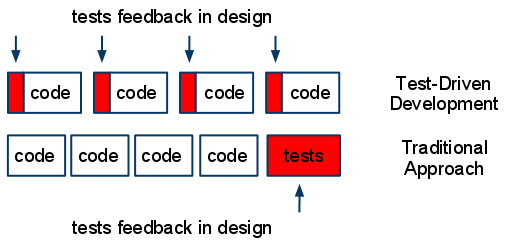
\includegraphics[scale=0.47]{findings/tdd-and-traditional.png}
  \caption{Feedback provido pela prática de TDD}
  \label{fig:tdd-feedback}
\end{figure}

A velocidade em que a prática de TDD dá \textit{feedback} ao desenvolvedor possibilita que o mesmo
tome decisões sobre o código enquanto o custo de mudança ainda é
baixo. O trabalho de Vanderburg \cite{vanderburg} também confirma este ponto.
Ele diz que TDD dá \textit{feedback} em questão de
minutos e, em questão de tempo, só é inferior à programação pareada. O gráfico,
baseado no trabalho dele, pode ser visto na Figura
\ref{fig:agile-feedback}.

\begin{figure}
  \centering
  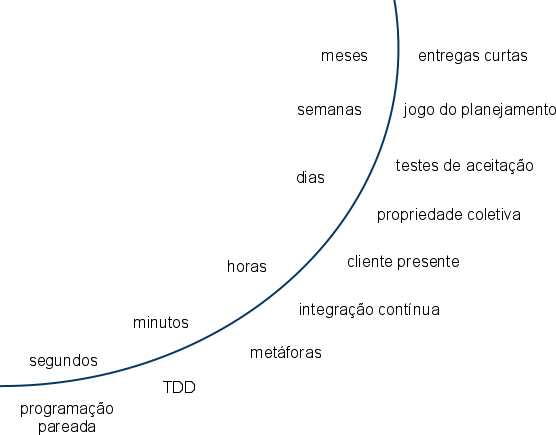
\includegraphics[scale=0.4]{agile-feedback-port}
  \caption{Práticas de XP e Tempo de \textit{Feedback} (baseado em \cite{vanderburg})}
  \label{fig:agile-feedback}
\end{figure}

Um participante comentou que, com o teste, você pode observar
e criticar o código que escreveu no momento logo após a escrita do mesmo.
E essa crítica, de forma contínua, faz com que o desenvolvedor acabe
por pensar constantemente no código que está produzindo:
\textit{"Quando você faz o teste, você vê logo o que não gostou do método daquele jeito (...), você
não percebe isso até que você use o teste."}

Diminuir o tempo entre o código e o teste também o ajuda a desenvolver código
que efetivamente resolve o problema. Segundo os participantes, na maneira tradicional, 
o desenvolvedor escreve muito código antes de saber se o mesmo funciona:
\textit{"[O teste] não é só uma especificação; ele tem que de fato funcionar. Então,
como você diminui muito o tempo entre escrever um programa que funcione e testar aquilo,
você consegue mais rápido ver se aquela parte pequena funciona ou não (...)"}


\subsection{Busca pela testabilidade}

Talvez o principal ponto pela qual a prática ajude os desenvolvedores no design de classes 
seja pela constante busca pela testabilidade. É possível inferir que, quando se 
começa a escrita do código pelo seu teste, o código de produção deve ser, necessariamente,
possível de testar.

Por outro lado, quando o código não é fácil de ser testado, os desenvolvedores
entendem isso como um mau cheiro de design de classes. Quando isso acontece,
os desenvolvedores geralmente tentam refatorar o código para possibilitar que
os mesmos sejam testados mais facilmente.

Um dos participantes, inclusive, afirmou que leva isso como uma regra:
se está difícil testar, é possível melhorar:
\textit{"Eu utilizo isso como uma regra: sempre que está muito complexo [o teste],
acho que nós temos que parar e refatorar, porque, na minha opinião, dá
pra ficar mais simples."}

Esse ponto, na verdade, já foi levantado antes por Feathers \cite{feathers-synergy}.
Quanto mais difícil for a escrita do teste, maior a chance da existência de
algum problema de design. Segundo ele, 
existe uma sinergia muito grande entre uma classe com alta testabilidade e um bom design: 
se o programador busca por testabilidade, acaba criando um bom design; se 
busca por um bom design, acaba escrevendo um design mais
testável.

Mas, os participantes foram ainda mais longe. Durante as entrevistas,
vários deles mencionaram diversos padrões que encontram nos testes,
e que os fazem pensar sobre os possíveis problemas de acoplamento,
coesão, falta de abstração, e etc, na classe que estão criando.
Esses padrões são melhor discutidos na Seção \ref{padroes-tdd}.


\section{Padrões de Feedback de DGT}
\label{padroes-tdd}

Na busca pela testabilidade, o desenvolvedor é encorajado a escrever um
código que seja facilmente testável. Códigos como esse possuem algumas
características interessantes, como a facilidade para invocar o comportamento
esperado, a não necessidade de pré-condições complicadas e a explicitação de
todas as dependências que a classe possui.

Outros autores já comentaram que 
TDD encoraja o programador a escrever componentes fracamente acoplados, de
maneira que eles possam ser testados de maneira isolada e, em um nível maior,
combinados com outros componentes.
Programar voltado para interfaces é uma prática de orientação a objetos há muito
tempo conhecida. Pensar em classes e dar maior foco à maneira com que
elas se relacionam do que com o modo que determinado comportamento será implementado
torna-se mais natural ao praticar TDD \cite{GOOS}. 

Como mencionado acima, grande parte do feedback que os testes
dão, acontecem no momento em que o programador encontra dificuldades para a
escrita do mesmo. Esta seção discute padrões levantados pelos praticantes
que os levam a crer que há um problema de design de classes no código
que está sendo testado.

\subsection{Coesão}

Quando um único método necessita de diversos testes para garantir seu comportamento,
indica que o método em questão é complexo e/ou possui diversas responsabilidades.
Esse padrão faz sentido já que códigos como esse possui geralmente diversos caminhos
diferentes e tendem a alterar muitos atributos internos do objeto, obrigando o desenvolvedor
a criar muitos testes, caso queira ter uma alta cobertura de testes nesta classe.
A esse padrão, demos o nome de \textbf{Muitos testes para um método}.

O mesmo pode ser entendido quando o desenvolvedor escreve muitos testes para a 
classe como um todo. Classes que expõem muitos métodos para o mundo de fora
também tendem a possuir muitas responsabilidades. Chamamos este padrão
de \textbf{Muitos testes para uma classe}.

Outro problema de coesão pode ser encontrado quando o programador
sente a necessidade de escrever cenários de teste muito grandes para uma
única classe ou método. É possível inferir que essa necessidade surge 
em códigos que lidam com muitos objetos e fazem muita coisa. Nomeamos
esse padrão de \textbf{Cenários muito grandes}.

Um padrão não explicitamente levantado pelos participantes, que notado
por nós, é quando o desenvolvedor sente a necessidade de se testar
um método que não é público. Métodos privados geralmente servem para 
transformar o método público em algo mais fácil de ler. Ao desejar
testá-lo de maneira isolada, o programador pode estar de frente com
um método que possua uma responsabilidade suficiente para ser
alocada em uma outra classe. A esse padrão, chamamos de 
\textbf{Testes em métodos que não são públicos}.

\subsection{Acoplamento}

Quando o programador faz uso abusivo de objetos dublês para testar uma
única classe, indica que a classe sob teste possui problemas
de acoplamento. É possível deduzir que uma classe que faz uso de muitos
objetos dublês depende de muitas classes, e portanto, tende a ser
uma classe instável. A esse padrão, demos o nome de \textbf{muitos mocks}.

Outro padrão percebido por nós é a criação de objetos dublês que não
são utilizados em alguns métodos de testes. Isso geralmente acontece quando
a classe é altamente acoplada, e o resultado da ação de uma dependência não
interfere na outra. Quando isso acontece, o programador acaba por escrever
conjuntos de testes, onde alguns deles lidam com parte dos objetos dublês,
enquanto a outra parte lida com a outra parte. Isso indica um alto acoplamento 
da classe, que precisa ser refatorado. A esse padrão demos o nome de
\textbf{mocks não utilizados}.


\subsection{Falta de abstração}

Quando, dado uma nova funcionalidade, o programador precisa propagar
a mesma alteração em diferentes testes, indica a falta de uma abstração 
correta para evitar a repetição do código que provavelmente existe. A 
esse padrão demos o nome de \textbf{mesma alteração em diferentes testes}.
Analogamente, o programador pode perceber a mesma coisa
quando ele começa a criar testes repetidos para entidades diferentes.
Chamamos esse padrão de \textbf{testes repetidos para entidades diferentes}.

Quando o desenvolvedor começa o teste e percebe que a interface pública da classe
que está sendo criada não está amigável, pode indicar que abstração
corrente não é clara o suficiente e poderia ser melhorada. A esse padrão,
chamamos de \textbf{interface nao amigavel}.

Outro padrão não mencionado explícitamente pelos participantes, 
é a existência da palavra \textit{"se"} no nome do teste. Testes que
possuem nomes como esse geralmente indicam a existência de um \textit{"if"} na implementação
do código de produção. Essas diversas condições podem, geralmente, ser refatoradas e,
através do uso de poliformismo, serem eliminadas. A falta de abstração nesse caso
é evidenciada pelo padrão \textbf{condicional no nome do teste}.

\section{Relação dos padrões com os princípios de design de classes}

% relacao com SOLID aqui

\section{Análise Quantitativa}

Conforme discutido no Capítulo \ref{cap:qualitativo-planejamento}, o teste
estatístico escolhido foi o Wilcoxon. Comparamos os valores encontrados
para as métricas de complexidade ciclomática, acoplamento eferente, falta
de coesão dos métodos, número de linhas por métodos, e quantidade de métodos
por classe nos códigos produzidos com TDD com as métricas colhidas dos
códigos produzidos sem TDD.
Devido ao problema que tivemos com os dados da academia, separamos a análise
dos dados, tanto das métricas de código, quanto dos especialistas, entre academia e indústria.

Nas sub-seções abaixo, discutimos os números encontrados.

\subsection{Métricas de código}

Na Tabela \ref{metricas-industria}, mostramos os \textit{p-values} encontrados para
a diferença entre códigos produzidos com e sem TDD na indústria. Pelos números, 
observamos que nem em nenhum exercício houveram diferenças nas métricas
de complexidade ciclomática e acoplamento eferente. Já a métrica de falta
de coesão dos métodos apresentou diferenças em dois exercícios (1 e 4). 
A diferença também apareceu na quantidade de linhas por método (exercício 4),
e quantidade de métodos (exercício 1). Ao olhar os dados de todos os exercícios
juntos, nenhuma métrica apontou uma diferença significativa.
Isso nos mostra que, ao menos quantitativamente, a prática de TDD não fez
diferença nas métricas de código.

\begin{table}
	\begin{tabular}{ | p{3cm} | p{2cm} | p{2cm} | p{2cm} | p{2cm} | p{2cm} |}
		\hline
		Exercício & Complexi- dade ciclomática & Acoplamento eferente & Falta de coesão dos métodos & Número de linhas por método 
		& Quantidade de métodos por classe \\
		\hline
		Exercício 1 &	0.8967	&	0.6741 &	2.04E-07* &	0.4962 &	2.99E-06* \\
		Exercício 2	& 0.7868	&	0.764 &	0.06132 &	0.9925 &	0.7501 \\
		Exercício 3	& 0.5463	&	0.9872 &	0.5471 &	0.7216 &	0.3972\\
		Exercício 4	& 0.2198	&	0.1361 &	0.04891* &	0.003286* &	0.9358\\
		\hline
		Todos &	0.8123	&	0.5604 &	0.3278 &	0.06814 &	0.5849\\
		\hline
	\end{tabular}
	\caption{\textit{P-values} encontrados para a diferença entre códigos com e sem TDD na indústria}
	\label{metricas-industria}
\end{table}

Na Tabela \ref{metricas-academia}, apontamos os \textit{p-values} das diferenças encontradas
entre códigos produzidos com e sem TDD na academia. As métricas de 
falta de coesão dos métodos e quantidade de métodos apresentaram
uma diferença significativa nos exercícios 1 e 4, respectivamente.
Ao olhar para todos os dados juntos, uma diferença significativa
apareceu também na métrica de acoplamento eferente.
Podemos então concluir que a prática de TDD também não afetou
o código produzido pelos participantes da academia.

\begin{table}
	\begin{tabular}{ | p{3cm} | p{2cm} | p{2cm} | p{2cm} | p{2cm} | p{2cm} |}
		\hline
		Exercício & Complexi- dade ciclomática & Acoplamento eferente & Falta de coesão dos métodos & Número de linhas por método 
		& Quantidade de métodos por classe \\
		\hline
			Exercício 1	& 0.2155	&	0.07085	& 0.00714* &	0.1721	& 0.008334*\\
			Exercício 2	& 0.7244	&	0.6744	& 1 &	0.3175 &	0.5591\\
			Exercício 3	& 0.7008	&	0.1014 &	0.5007	& 0.4292	& 0.8687\\
			Exercício 4	& 0.343	&	0.7131 &	0.7735	& 0.7833	& 0.5522\\
		\hline
			Todos &	0.254	&	0.007676* & 0.351 & 0.2668 & 0.1706\\
		\hline
	\end{tabular}
	\caption{\textit{P-values} encontrados para a diferença entre códigos com e sem TDD na academia}
	\label{metricas-academia}
\end{table}

\subsection{Especialistas}

Ambos os especialistas não encontraram diferenças entre códigos produzidos
com e sem TDD, tanto na indústria, quanto na academia. Nas Tabelas 
\ref{tab:especialistas-industria} e \ref{tab:especialistas-academia},
mostramos os \textit{p-values} encontrados para a diferença de avaliação dos especialistas
entre códigos produzidos com e sem TDD na indústria e academia, respectivamente.


\begin{table}[h!]
	\begin{tabular}{| p{5cm} | c | c | c | }
		\hline
		Especialista & Design & Testabilidade & Simplicidade\\
		\hline
		Especialista 1 &	0.4263 &	0.5235 &	0.332\\
		Especialista 2 &	0.7447 &	0.4591 &	0.9044\\
		\hline
	\end{tabular}
	\caption{\textit{P-values} encontrados para a diferença entre as análises dos especialistas com e sem TDD na indústria}
	\label{tab:especialistas-industria}
\end{table}

\begin{table}[h!]
	\begin{tabular}{| p{5cm} | c | c | c | }
		\hline
		Especialista & Design & Testabilidade & Simplicidade\\
		\hline
		Especialista 1	& 0.8795 &	NA	& 0.4222\\
		Especialista 2	& 0.88	& 0.5519 &	0.88\\
		\hline
	\end{tabular}
	\caption{\textit{P-values} encontrados para a diferença entre as análises dos especialistas com e sem TDD na academia}
	\label{tab:especialistas-academia}
\end{table}
